%%%%%%%%%%%%%%%%%%%%%%%%%%%%%%%%%%%%%%%%%
% University/School Laboratory Report
% LaTeX Template
% Version 3.1 (25/3/14)
%
% This template has been downloaded from:
% http://www.LaTeXTemplates.com
%
% Original author:
% Linux and Unix Users Group at Virginia Tech Wiki 
% (https://vtluug.org/wiki/Example_LaTeX_chem_lab_report)
%
% License:
% CC BY-NC-SA 3.0 (http://creativecommons.org/licenses/by-nc-sa/3.0/)
%
%%%%%%%%%%%%%%%%%%%%%%%%%%%%%%%%%%%%%%%%%

%----------------------------------------------------------------------------------------
%	PACKAGES AND DOCUMENT CONFIGURATIONS
%----------------------------------------------------------------------------------------

\documentclass{ctexart}

\usepackage[version=3]{mhchem} % Package for chemical equation typesetting
\usepackage{siunitx} % Provides the \SI{}{} and \si{} command for typesetting SI units
\usepackage{graphicx} % Required for the inclusion of images
\usepackage{natbib} % Required to change bibliography style to APA
\usepackage{amsmath} % Required for some math elements 
%\usepackage{showframe} % for showing page frames


\setlength\parindent{0pt} % Removes all indentation from paragraphs

\renewcommand{\labelenumi}{\alph{enumi}.} % Make numbering in the enumerate environment by letter rather than number (e.g. section 6)

%\usepackage{times} % Uncomment to use the Times New Roman font

%==========pesusdo codes
\usepackage[linesnumbered,boxed]{algorithm2e}
%\renewcommand{\algorithmcfname}{算法}
\renewcommand{\repeat}{Repeat}

%==========citation===========
%\usepackage{cite}
\usepackage{url}


% ==========添加首行缩进,两个字符===========
\usepackage{indentfirst}
\setlength{\parindent}{2em}
% ==========强制图片位置===========
\usepackage{float}

% ==========特殊数学符号===========
\usepackage{mathtools}
\usepackage{dsfont}
\usepackage{amsfonts}
% ==========列表===========
\usepackage{enumerate}

%----------------------------------------------------------------------------------------
%	DOCUMENT INFORMATION
%----------------------------------------------------------------------------------------

\title{EM及其特例GMM} % Title

%\author{fengmi \textsc{Feng}} % Author name

\author{Mia Feng} % Author name

\date{\today} % Date for the report

\begin{document}

\maketitle % Insert the title, author and date

%\begin{center}
%\begin{tabular}{l r}
%Date Performed: & January 1, 2012 \\ % Date the experiment was performed
%Partners: & James Smith \\ % Partner names
%& Mary Smith \\
%Instructor: & Professor Smith % Instructor/supervisor
%\end{tabular}
%\end{center}

% If you wish to include an abstract, uncomment the lines below
% \begin{abstract}
% Abstract text
% \end{abstract}

%----------------------------------------------------------------------------------------
%	SECTION 1
%----------------------------------------------------------------------------------------

\section{概述}
EM算法:无监督,density estimation模型。用于含有latent variable的概率模型的极大似然估计(MLE)。算法对初始值敏感。因为latent variable的不可观测性,所以似然函数最大化难以处理,代替的,我们把难于处理的最大化似然函数问题用一个易于最大化的序列(对数似然函数序列)取代,其极限是原始问题的解。原本的关于参数$\theta$的最优化问题被离散到一些$L\big(\theta\big)$对数似然序列上求解。虽然最终可以收敛到$L\big(\theta\big)$的稳定点,但是不一定保证能收敛到极大值点(因为不是关于参数估计序列$\theta$的收敛),即最终结果可能陷入局部最优。算法分为E(expectation)步和M(maximization)步,E步求latent variable的条件概率分布的期望,M步通过最大化期望更新参数。迭代直至算法收敛(参数改动小于某个阈值或者期望变化小于某个阈值)

GMM假设样本从多个高斯分布中生成,只是EM后验分布取混合高斯分布的一种特例。基于中心极限定理以及Gaussian Distribution的良好性质,GMM算法应用较广。

作为无监督学习算法,GMM与$k$-means相比是类似的。GMM-E步中对高斯分量的响应度相当于$k$-means中的距离计算,GMM-M根据响应度计算高斯分量参数相当于$k$-means中计算分类点的位置。然后都是不断迭代达到最优\cite{gmm:kmeans}。
%To determine the atomic weight of magnesium via its reaction with oxygen and to study the stoichiometry of the reaction (as defined in \ref{definitions}):

求解目标:聚类,每个样本点给出其可能来自潜在变量$i$的概率。

求解思路:最大化关于latent variable的对数似然函数,取对数似然函数最大时对应的参数$\theta$作为未知变量的解。最终根据$\theta^*$求得样本来自latent variable的评分(概率)。

求解方法:MLE(Maximum likelihood estimator)。

Tips:确定了响应度之后,参数更新有显式的函数表达

Preliminary:Jensen's inequality,


% If you have more than one objective, uncomment the below:
%\begin{description}
%\item[First Objective] \hfill \\
%Objective 1 text
%\item[Second Objective] \hfill \\
%Objective 2 text

\subsection{EM算法}
\label{derivations}
重点在于写出完全数据的对数似然函数的期望(之所以称为完全,是假定补充了latent variable之后的数据),即$Q$函数
\begin{description}
\item[$Q$函数\cite{LiHang:Statistic}]
完全数据的对数似然函数$\log P\big(Y,Z|\theta\big)$关于在给定观测数据$Y$和当前参数$\theta^{\left(i\right)}$下对未观测数据$Z$的条件概率分布$\log P\big(Y,Z|\theta^{\left(i\right)}\big)$的期望
\begin{equation}
Q\big(\theta,\theta^{\left(i\right)}\big)=\mathbb{E}_Z\left[\log P\big(Y,Z|\theta\big)|Y, \theta^{\left(i\right)}\right]
\end{equation}

\item[Jensen's Inequality]
当函数是convex function时,期望的函数值小于等于函数值的期望
\begin{equation}
\mathbb{E}\big[f\big(X\big)\big]\leq f\big(\mathbb X\big)
\end{equation}
\end{description}
推导对$Q$函数利用Jensen's Inequality,参见page158-159\cite{LiHang:Statistic},收敛性证明参见page161-162\cite{LiHang:Statistic}。

\begin{figure}[H]
\begin{center}
\includegraphics[width=0.8\textwidth]{fig/em-derive1.jpg} 
\includegraphics[width=0.8\textwidth]{fig/em-derive2.jpg} 
\caption{EM推导}
\end{center}
\end{figure}

\begin{figure}[H]
\begin{center}
\includegraphics[width=0.8\textwidth]{fig/em-converge1.jpg} 
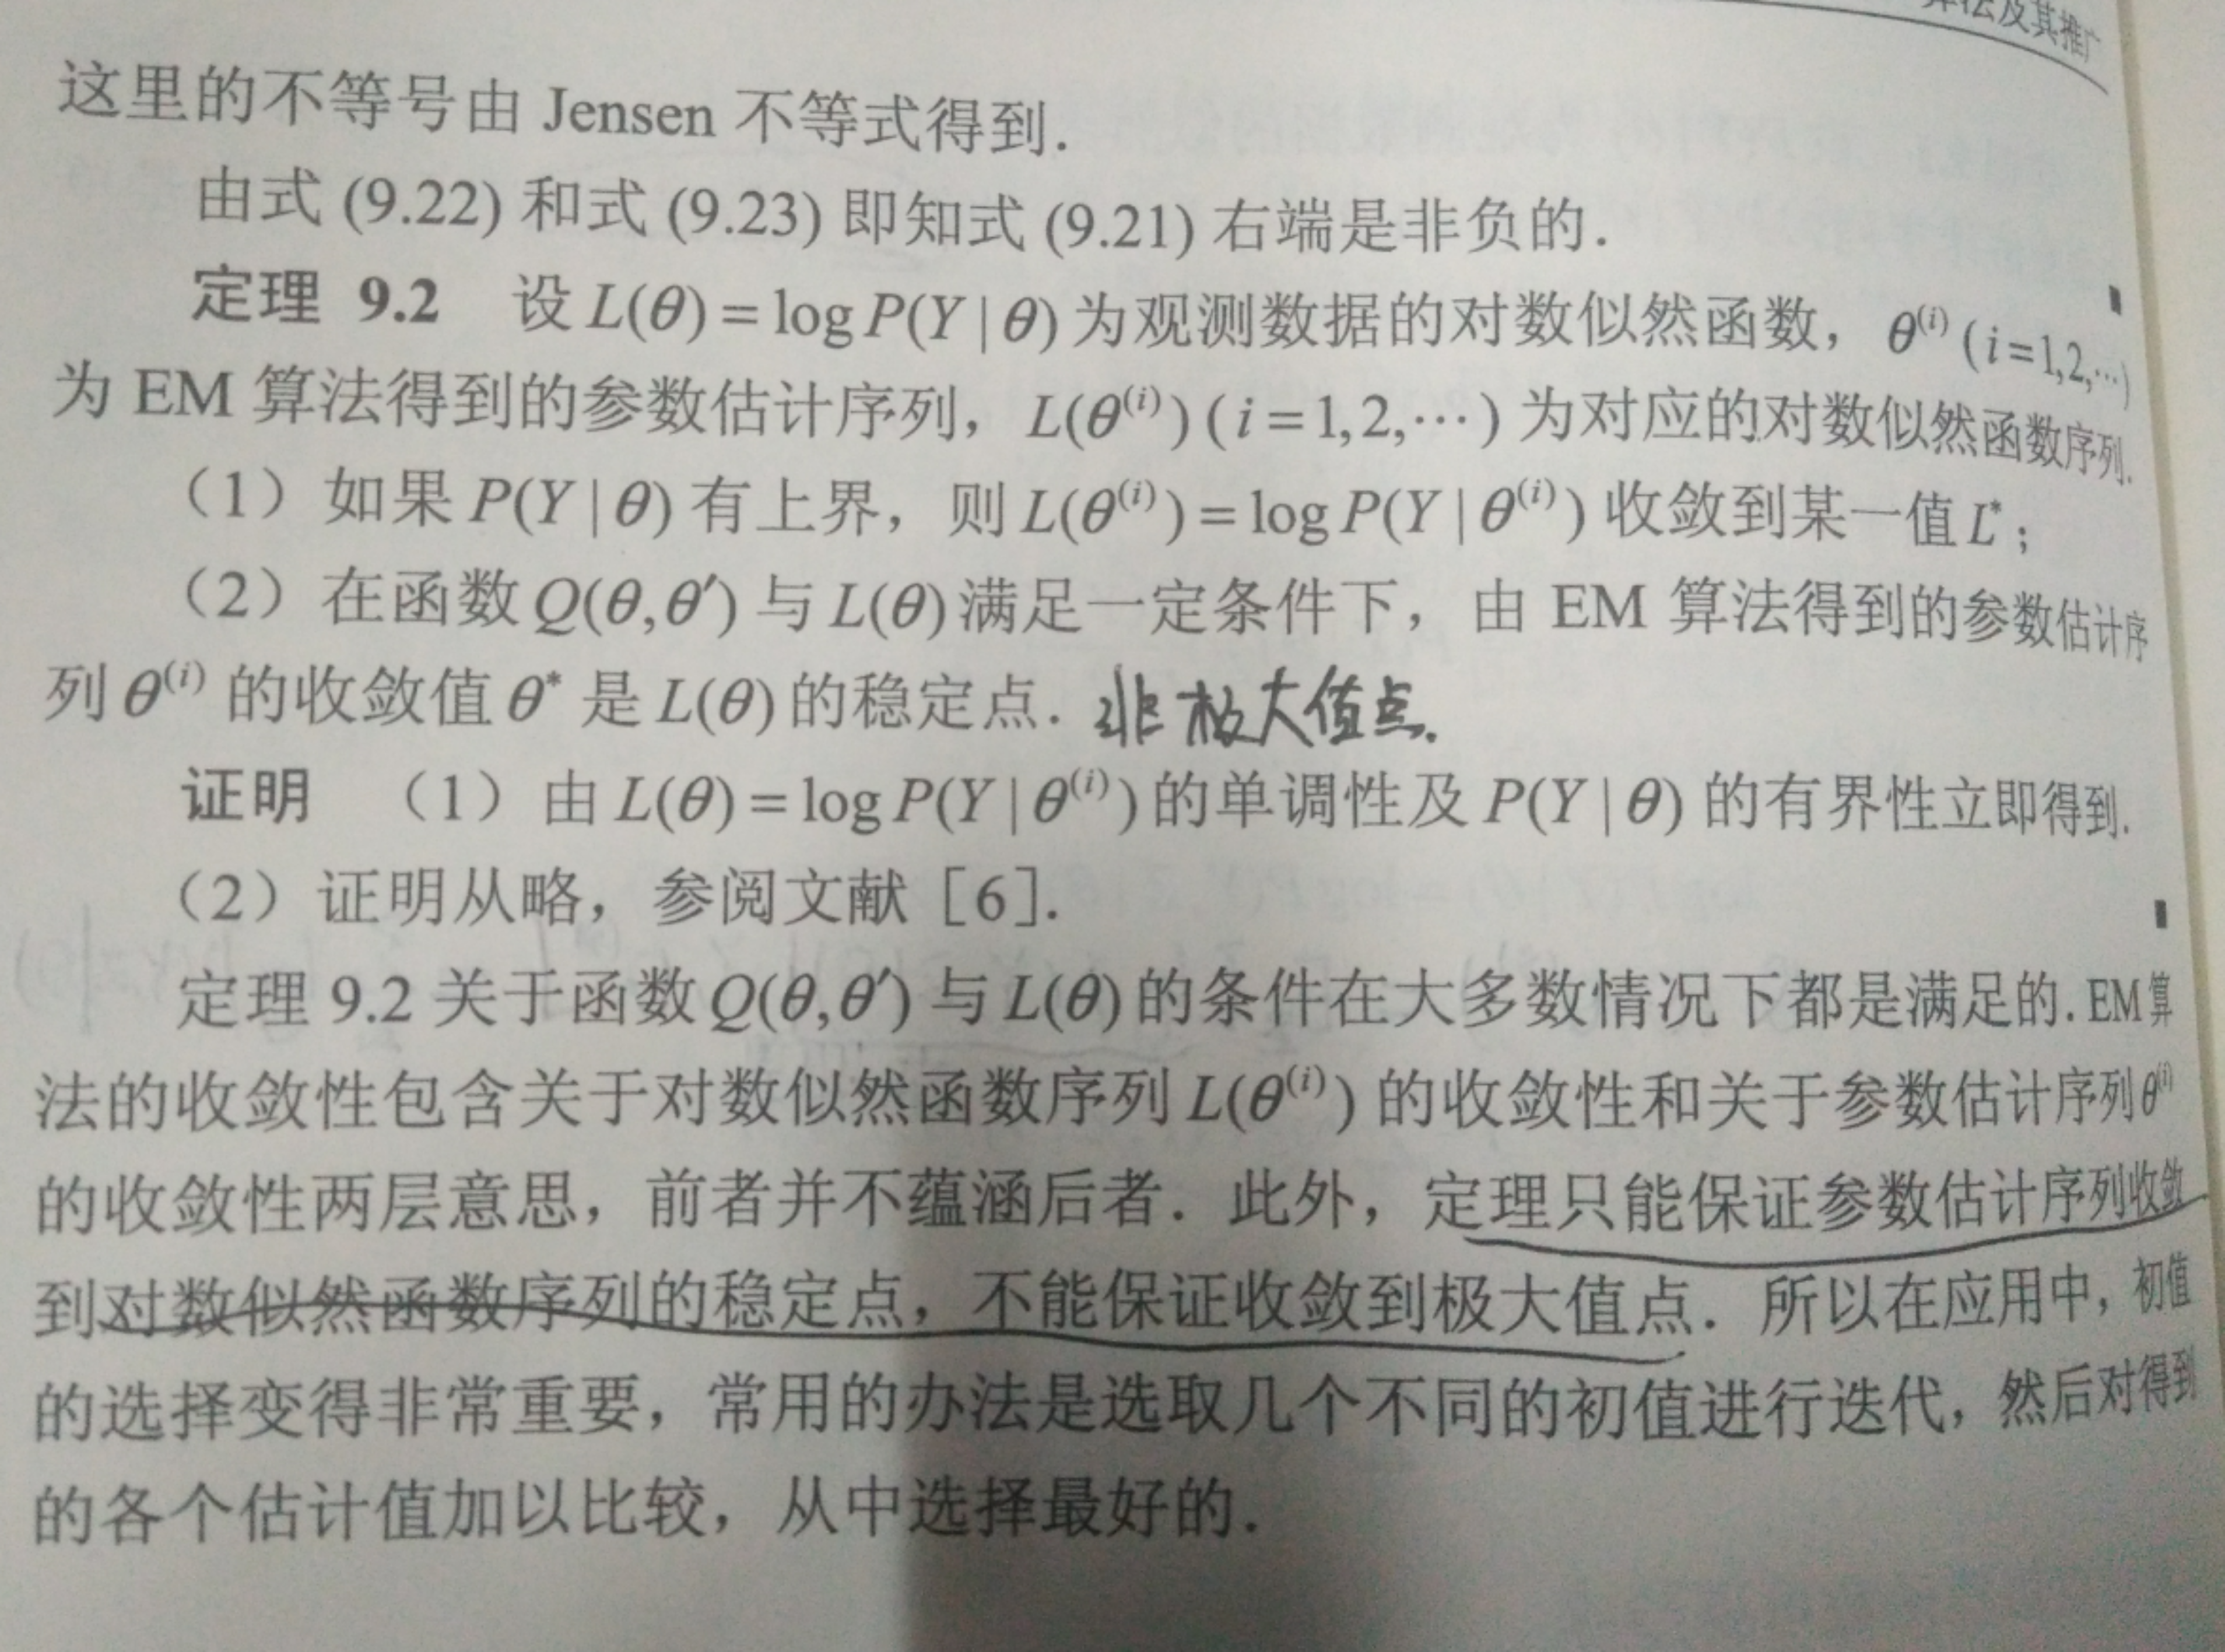
\includegraphics[width=0.8\textwidth]{fig/em-converge2.png} 
\caption{EM收敛性证明}
\end{center}
\end{figure}


\subsection{GMM算法}
\label{gmm}
EM的特例,假设样本来自混合高斯分布(多个高斯分布),latent variable服从multinomial分布(这是自然的,是为了标志数据从哪个分布产生,自然只有0,1两种可能性,多个高斯成分均匀混合对应multinomial)。算法其实也可以用别的方法求极值,EM只是一种求解方法。
\begin{description}
\item[高斯混合分布]
$k$个高斯分布均匀混合得到的概率分布模型。
\begin{equation}
P\big(y|\theta \big)=\sum\limits_{k=1}^{K}\alpha_k\phi\big(y|\theta_k\big)
\end{equation}
其中,系数$\alpha_k\ge0,\sum\limits_{k=1}^{K}\alpha_k=1$
注意这里$P$是PDF(probability distribution function)而非CDF(cumulative distribution function)。高斯分布的钟形图是PDF,混合高斯分布的PDF是由各高斯成分线性叠加形成的。这也解释了系数$\alpha_k$为什么一定小于1且加和为1,因为GMM整体的PDF积分才为1。

\end{description}
李航的书上没有具体求各项的导数,这里用了CS229-notes中的推导,并补充了讲义中关于方差的更新公式的推导。
\begin{figure}[H]
\begin{center}
\includegraphics[width=0.8\textwidth]{fig/gmm1.jpg}  
\caption{GMM算法推导-1}
\end{center}
\end{figure}
\begin{figure}[H]
\begin{center}
\includegraphics[width=0.8\textwidth]{fig/gmm2.jpg}  
\caption{GMM算法推导-2}
\end{center}
\end{figure}

\begin{figure}[H]
\begin{center}
\includegraphics[width=0.8\textwidth]{fig/gmm3.jpg}  
\caption{GMM算法推导-3}
\end{center}
\end{figure}

%----------------------------------------------------------------------------------------
%	SECTION 2
%----------------------------------------------------------------------------------------

\section{算法实现}
\begin{figure}[H]
\begin{center}
\includegraphics[width=0.8\textwidth]{fig/steps.png}  
\caption{GMM算法步骤}
\end{center}
\end{figure}

%----------------------------------------------------------------------------------------
%	SECTION 3
%----------------------------------------------------------------------------------------
%
\section{Implementation}
聚类测试:数据用四个二元高斯分布混合生成。
但是在更新方差的时候总会出现奇异矩阵,这样的话没法更新。还不知道原因是什么。暂时将方差固定,但是结果还不是很好,留待解决
%\begin{figure}[H]
%\begin{center}
%\includegraphics[width=0.8\textwidth]{fig/raw.png} % Include the image placeholder.png
%\caption{训练数据}
%\end{center}
%\end{figure}
%
%\begin{figure}[H]
%\begin{center}
%\includegraphics[width=0.8\textwidth]{fig/iter-01.png} % Include the image placeholder.png
%\caption{kmeans运行结果,iter=1,$k$=4。菱形标记聚类中心,点标记数据}
%\end{center}
%\end{figure}
%
%
%\begin{figure}[H]
%\begin{center}
%\includegraphics[width=0.8\textwidth]{fig/iter-02.png} % Include the image placeholder.png
%\caption{kmeans运行结果,iter=2,$k$=4。菱形标记聚类中心,点标记数据}
%\end{center}
%\end{figure}
%
%
%\begin{figure}[H]
%\begin{center}
%\includegraphics[width=0.8\textwidth]{fig/iter-03.png} % Include the image placeholder.png
%\caption{kmeans运行结果,iter=3,$k$=4。菱形标记聚类中心,点标记数据}
%\end{center}
%\end{figure}

%%----------------------------------------------------------------------------------------
%%	SECTION 4
%%----------------------------------------------------------------------------------------
%
%\section{Results and Conclusions}
%
%The atomic weight of magnesium is concluded to be \SI{24}{\gram\per\mol}, as determined by the stoichiometry of its chemical combination with oxygen. This result is in agreement with the accepted value.
%
%\begin{figure}[h]
%\begin{center}
%\includegraphics[width=0.65\textwidth]{placeholder} % Include the image placeholder.png
%\caption{Partial Gradient of $L_\big(\theta \big)$}
%\end{center}
%\end{figure}
%
%%----------------------------------------------------------------------------------------
%%	SECTION 5
%%----------------------------------------------------------------------------------------
%
%\section{Discussion of Experimental Uncertainty}
%
%The accepted value (periodic table) is \SI{24.3}{\gram\per\mole} \cite{Smith:2012qr}. The percentage discrepancy between the accepted value and the result obtained here is 1.3\%. Because only a single measurement was made, it is not possible to calculate an estimated standard deviation.
%
%The most obvious source of experimental uncertainty is the limited precision of the balance. Other potential sources of experimental uncertainty are: the reaction might not be complete; if not enough time was allowed for total oxidation, less than complete oxidation of the magnesium might have, in part, reacted with nitrogen in the air (incorrect reaction); the magnesium oxide might have absorbed water from the air, and thus weigh ``too much." Because the result obtained is close to the accepted value it is possible that some of these experimental uncertainties have fortuitously cancelled one another.
%
%%----------------------------------------------------------------------------------------
%%	SECTION 6
%%----------------------------------------------------------------------------------------
%
%\section{Answers to Definitions}
%
%\begin{enumerate}
%\begin{item}
%The \emph{atomic weight of an element} is the relative weight of one of its atoms compared to C-12 with a weight of 12.0000000$\ldots$, hydrogen with a weight of 1.008, to oxygen with a weight of 16.00. Atomic weight is also the average weight of all the atoms of that element as they occur in nature.
%\end{item}
%\begin{item}
%The \emph{units of atomic weight} are two-fold, with an identical numerical value. They are g/mole of atoms (or just g/mol) or amu/atom.
%\end{item}
%\begin{item}
%\emph{Percentage discrepancy} between an accepted (literature) value and an experimental value is
%\begin{equation*}
%\frac{\mathrm{experimental\;result} - \mathrm{accepted\;result}}{\mathrm{accepted\;result}}
%\end{equation*}
%\end{item}
%\end{enumerate}

%----------------------------------------------------------------------------------------
%	BIBLIOGRAPHY
%----------------------------------------------------------------------------------------
%
% 注意一定要在文中引用才不会出错(至少引用一个)
\bibliographystyle{plain}
\bibliography{bib//gmm}

%----------------------------------------------------------------------------------------


\end{document}